\documentclass{article}
\usepackage{amsmath}
\usepackage{amssymb}
\usepackage{graphicx}
\usepackage{hyperref}
\usepackage[version=4]{mhchem}

\title{Problem 5}
\date{}

\begin{document}
\maketitle

\section*{Problem}
In \(\triangle A B C\), angle \(C\) is a right angle. \(A C\) and \(B C\) are each equal to 1. \(D\) is the midpoint of \(A C . B D\) is drawn, and a line perpendicular to \(B D\) at \(P\) is drawn from \(C\). Find the distance from \(P\) to the intersection of the medians of \(\triangle A B C\).\\
\centering
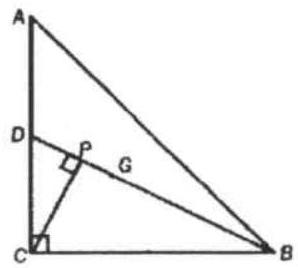
\includegraphics[width=\textwidth]{images/problem_image_1.jpg}

\section*{Solution}
\(\frac{1}{15} \sqrt{5}\).\\
Applying the Pythagorean Theorem to \(\triangle D C B\) gives us\\
\((D C)^{2}+(C B)^{2}=(D B)^{2}\).\\
\(1 / 4+1=(D B)^{2}, D B=\frac{1}{2} \sqrt{5}\).\\
Since the centroid of a triangle trisects each of the medians,\\
\(D G=\frac{1}{3} D B=\frac{1}{3}\left(\frac{1}{2} \sqrt{5}\right)=\frac{1}{6} \sqrt{5}\)\\
Consider right \(\triangle D C B\) where \(C P\) is the altitude drawn upon the hypotenuse.\\
Therefore, \(D B / D C=D C / D P . \frac{\frac{1}{2} \sqrt{5}}{\frac{1}{2}}=\frac{\frac{1}{2}}{D P}, D P=\frac{\sqrt{5}}{10}\)\\
\centering
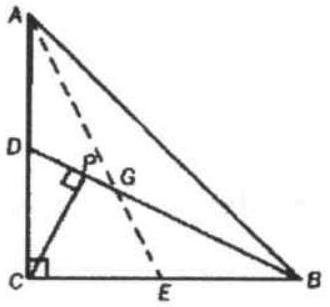
\includegraphics[width=\textwidth]{images/reasoning_image_1.jpg}

Thus, \(P G=D G-D P\), and \(P G=\frac{1}{6} \sqrt{5}-\frac{1}{10} \sqrt{5}=\frac{1}{15} \sqrt{5}\).

\end{document}
